\chapter{MVP Boundaries, UML Schematics, and Architectural Topologies}
\label{chap:architecture}
\setlength{\parskip}{1em}

\section{Minimum Viable Product (MVP) Trajectory}
The minimum viable product (MVP) scope for Lectura was deliberately aggressively constrained to physically validate the fundamental generative hypothesis without succumbing to feature bloat. The defined strict perimeter required for a successful MVP launch encapsulates: secure user instantiation and credentials oversight, raw multimedia payload submission, real-time spatial transcript extraction, automated synthesis of high-order pedagogical artifacts (summaries, algorithmic quizzes, flashcards, and strictly templated presentations), and a functional, persistent frontend knowledge library. Advanced telemetry plotting and heavy offline native sync logic were explicitly deferred to future release candidate phases to ensure developmental velocity.

\section{System Architecture Overview}
The overarching physical schema is comprehensively documented within Figure~\ref{fig:sys_architecture}. Lectura effectively enforces a rigid three-tier distributive topology: an aggressive Client Presentation Layer governed entirely by React, an Asynchronous Application Logic Layer marshaled in Go, and a deep Persistent Data/Generative execution tier driven by PostgreSQL, Redis, and Google’s Gemini API matrices.

\begin{figure}[htbp]
\centering
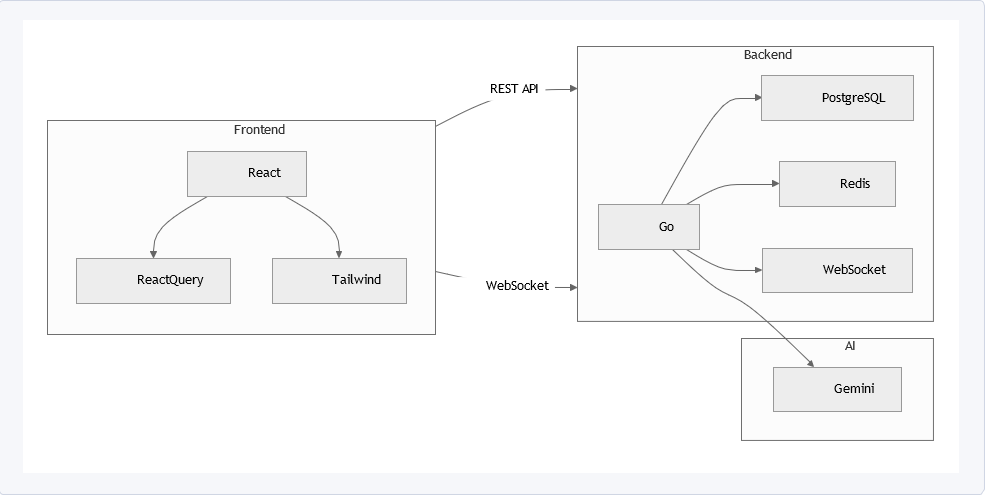
\includegraphics[width=\textwidth]{chapters/chapter05/images/sys_architecture.png}
\caption{System Architecture Diagram mapping the three-tier distributive environment.}
\label{fig:sys_architecture}
\end{figure}

\section{Use Case Interaction Diagram}
Figure~\ref{fig:use_case} aggressively isolates the interaction vectors defining the application boundary. The structural map explicitly differentiates behavioral capabilities granted to Guest proxies versus Authenticated User nodes, subsequently mapping their explicit triggers against the automated System inference logic.

\begin{figure}[htbp]
\centering
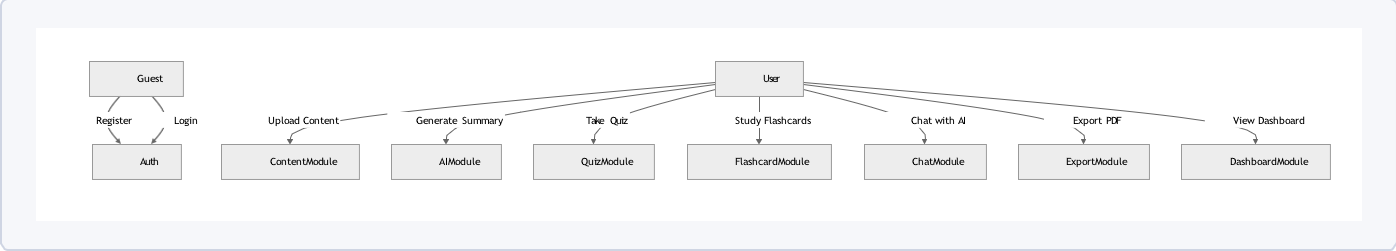
\includegraphics[width=0.9\textwidth]{chapters/chapter05/images/image2.png}
\caption{Interaction parameters between Authenticated Actor nodes and System functionalities.}
\label{fig:use_case}
\end{figure}

\section{Asynchronous Content Generation Sequence}
Given the asynchronous brutality of invoking external LLM APIs, Figure~\ref{fig:sequence_gen} chronicles the exact chronological execution path. It visually illustrates the linear instantiation logic triggering from the user client, parsing through the Go orchestrator, decoupling via the Redis worker pool queue, resolving at the Gemini API terminal, and structurally concluding with a WebSocket spatial notification burst driving back to the React UI.

\begin{figure}[htbp]
\centering
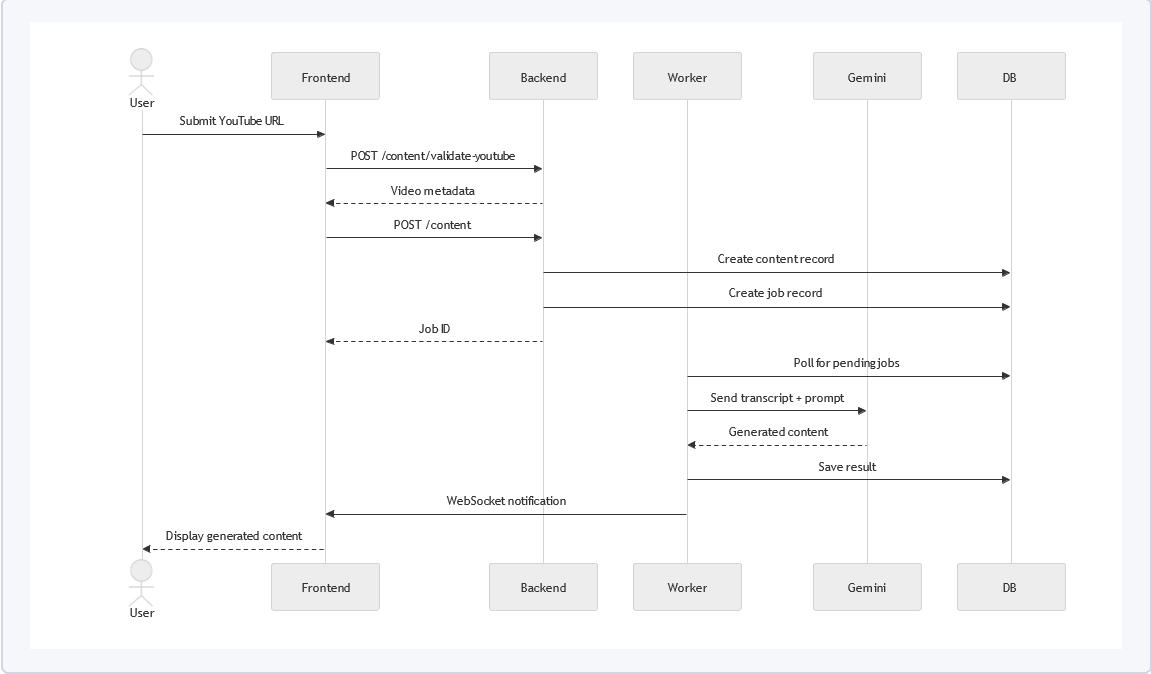
\includegraphics[width=\textwidth]{chapters/chapter05/images/image3.png}
\caption{Asynchronous Chronological Sequence mapping the external LLM invocation cycle.}
\label{fig:sequence_gen}
\end{figure}

\section{Authentication Telemetry Sequence}
To ensure absolute network security, Figure~\ref{fig:auth_matrix} dissects the cryptographic authentication vector. It maps the explicit physical handshake occurring during OAuth onboarding, the execution of JWT credential signing, the provisioning of hyper-secure HttpOnly refresh tokens, and the subsequent aggressive client validation cycles required to penetrate secure backend APIs.

\begin{figure}[htbp]
\centering
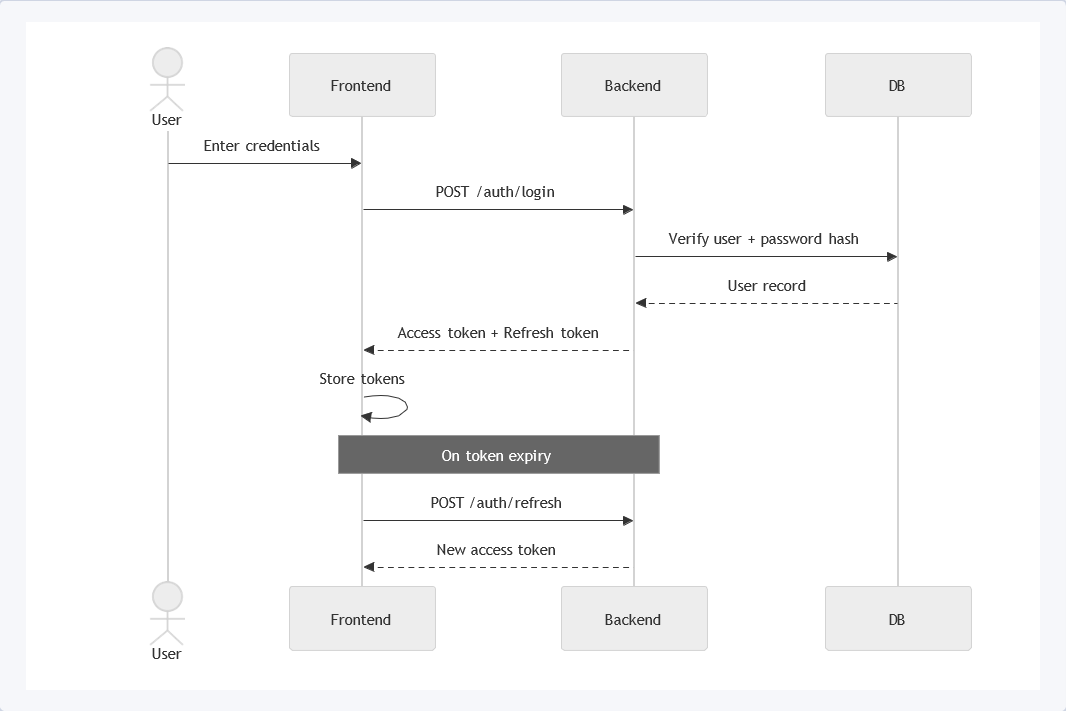
\includegraphics[width=\textwidth]{chapters/chapter05/images/image4.png}
\caption{Cryptographic Authentication Matrix mapping JWT handshake topologies.}
\label{fig:auth_matrix}
\end{figure}

\section{Entity Relationship Relational Logic}
The strict algebraic intersections defining the data warehousing infrastructure are codified in Figure~\ref{fig:er_matrix}. It explicitly maps the primary foreign key vectors enforcing referential integrity between localized Users, the raw extracted Content strings, and the heavily abstracted JSON permutations stored natively across the Summaries, Quizzes, Presentations, and Flashcards ledgers.

\subsection{Mathematical Database Indexing Complexity: JSONB vs B-Tree}
A pivotal architectural decision involves persisting chaotic, deeply nested LLM outputs (such as dynamic quiz questions containing variable arrays of distractor answers) inside a historically rigid Relational Database Management System (RDBMS) like PostgreSQL. To maintain $O(\log n)$ search limits while avoiding schema-breaking normalized table sprawling, Lectura relies heavily upon the JSONB object type.

Unlike raw text formatting, the JSONB paradigm decomposes and stores payload data in a mathematically optimized binary superstructure. This allows PostgreSQL to deploy Generalized Inverted Indexes (GIN) across the deeply nested heuristic keys. If the backend needs to physically extract all quizzes generated beneath a specific user UUID that contain specifically failed question types, the GIN index operates fundamentally as a bipartite graph search without requiring a full sequential table scan $O(n)$.

The traditional B-Tree index, which Lectura applies to standard strict columns like \texttt{created\_at} or \texttt{user\_id}, calculates search topography using logarithmic branching logic:

\begin{equation}
    T_{\text{search}} \approx O(\log_b n)
\end{equation}

Where $b$ represents the branch factor limit of the specific index page, and $n$ represents the total rows. However, a B-Tree categorically fails when required to traverse varying nested depths of an unstructured JSON array. By converting the LLM payload into a strict JSONB binary map and overlaying a GIN index, Lectura effectively collapses unstructured extraction searches to near localized $O(1)$ lookup times for specific keys, mathematically isolating generative schema fluidity from dragging down traditional relational velocity.

\begin{figure}[htbp]
\centering
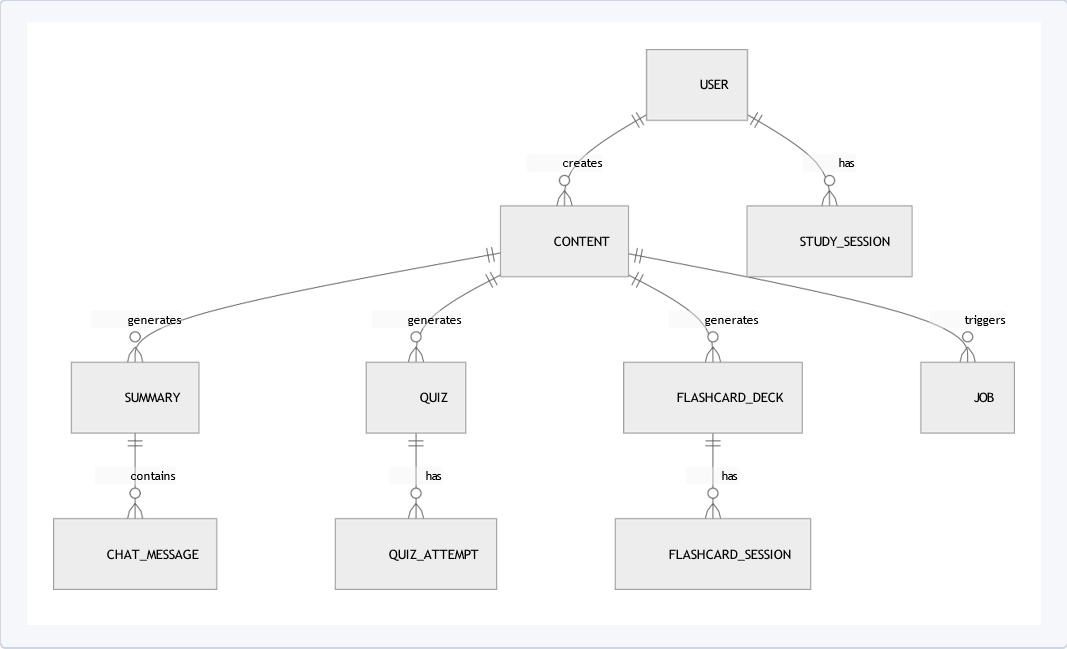
\includegraphics[width=0.9\textwidth]{chapters/chapter05/images/image5.png}
\caption{Entity Relationship Matrix defining the normalized PostgreSQL persistence layer.}
\label{fig:er_matrix}
\end{figure}

\section{Decoupled Component Schematics}
The macro-scale component architecture radically decouples execution loops. The frontend presentation layer mathematically insulates the internal states of the Authentication interceptors, the Raw Media Ingestors, and the Artifact Renderers. Concurrently, the Go backend forces a strict dependency injection model separating API Router meshes, distinct Handler endpoints, abstract Business Services, physical Database Repositories, and the autonomous Worker Pool loops.

\section{Advanced Worker Pool Engineering}
The inclusion of an insulated worker pool defines the crux of the backend resilience. By deliberately shielding the execution thread from the fundamental volatility of the external generation APIs, the worker pool mathematically guarantees extremely aggressive concurrency scaling, the absolute isolation of long-tail computational lags, intelligent backoff and retry mechanisms, and the strict enforcement of rate-limiting physics to prevent infrastructure throttling.